\chapter{Universal Clues in the Ballot Box}
\label{chap4}

In the previous chapter, we established a solid empirical foundation by curating and analyzing election data from diverse democratic systems across the globe. We now shift our focus towards uncovering universal patterns in these data. 

\section{The Allure of Universality: Why Physicists Chase Patterns in Politics}

One of the cornerstones of democratic societies is that governance must be based on an expression of the collective will of the citizens. The institution of elections is central to the operational success of this system. Elections to public offices are the best-documented instances of collective decision-making by humans, whose outcome is determined by multiple agents interacting over a range of spatial and temporal scales. These features make elections an interesting test-bed for statistical physics whose key lesson is that a multitude of complex interactions between microscopic units of a system can manifest into robust, {\it universal} behavior at a macroscopic level \cite{anderson1972more,strogatz2022fifty,CasForLor2009, JedSzn2019, MigTor2020, galam2012, brams2008, ForMacRed2013, Bouchaud2023, SenCha2014, PerJorRan2017,JusHolKan2022,redner2019reality}. A collection of gas molecules or spins are examples that display such emergent macroscopic features \cite{REI65}, and so are complex processes such as earthquakes \cite{Corral2004,Corral2006} and financial markets \cite{PleGopRos1999}. In the context of elections, such universal behaviors serve to distill the complexities of electoral dynamics into understandable and predictive frameworks and safeguard its integrity.

The implications of such universality would be profound. From a theoretical standpoint, it would suggest that the act of electoral competition itself—the fundamental process of competing candidates vying for votes—contains intrinsic statistical properties that transcend the particularities of any given election. From a practical perspective, universal patterns could provide benchmarks against which to evaluate the health and integrity of democratic processes worldwide.

\subsection{A History of Near Misses: Previous Expeditions for Electoral Universals}

Unsurprisingly, the possibility of universality in elections attracts significant research attention \cite{CosAlmAnd1999, ForCas2007, BorBou2010, mantovani2011scaling, BokSzaVat2018, ChaMitFor2013, hosel2019universality}. Several works have studied and proposed models for ({\it a}) the distribution $q(\sigma)$ of the fraction of votes $\sigma$ obtained by candidates (or the vote share), and ({\it b}) distribution $g(\tau)$ of voter turnout $\tau$. While $\sigma$ is indicative of popularity, $\tau$ indicates the scale of the election. Though some universality has been observed in $q(\sigma)$ or $g(\tau)$ within a single country \cite{ForCas2007,CosAlmAnd1999, BorBou2010} or in countries with similar election protocols \cite{ForCas2007, ChaMitFor2013}, deviations from claimed universalities have also been reported \cite{ChaMitFor2013, Kon2017,Kon2019, CalCroAnt2015, BorRayBou2012} due to variations in the size (scale) of electoral districts and weak party associations. Though voting patterns tend to display spatial correlations \cite{FerSucRam2014, BraDeA2017,MicIlkAtt2021,MorHisNak2019}, it is not known to be universal. Despite the availability of enormous election data and persistent attempts, a robust and universal emergent behavior, valid across different scales and countries with vastly different election protocols, is yet to be demonstrated.

The primary limitations of previous approaches include scale dependency (distributions vary significantly when comparing different electoral unit sizes), system specificity (patterns observed in one electoral system rarely translate to systems with different party structures or voting rules), and lack of robustness (proposed universalities typically fail when tested against geographically and culturally diverse electoral data).

These limitations have created a gap in our understanding—we lack a truly universal pattern valid across different scales, countries, and electoral systems. In this chapter, we aim to fill this gap by exploring a different combination of electoral variables that may yield robust universality.

\section{The Chosen Variables: Margin of Victory (M) and Voter Turnout (T)}

Among the many metrics that characterize democratic elections, we focus on two fundamental variables: the margin of victory and voter turnout. These variables capture essential aspects of electoral contests while being measurable across virtually all democratic systems, regardless of the specific rules and structures in place.

\subsection{Why These Two Variables?}

A template of a basic electoral process is as follows. At each electoral unit, candidates compete against each other to win the votes of the electorate, who can cast their vote in favor of only one of the candidates. The candidate securing the largest number of polled votes is declared the winner. This represents the core process in many electoral systems. It is the standard first-past-the-post system followed in many countries, e.g., India, the UK, and the USA. In an instant-run-off system (such as in Australia) or two-round run-offs (such as in France), the final run-off round boils down to this template. Typically, national or regional elections following this template consist of many electoral units made up of polling booths, precincts, constituencies, or counties. These units set a size scale in terms of the number of electorates -- polling booth represents the smallest scale, while a constituency (subsuming many polling booths) represents the largest scale. For our analysis, an ``election'' could be either a national, regional, or even a city-level electoral process encompassing $N$ electoral units, and each unit could be a polling booth, county, or constituency.

In any such election, an informative indicator of the degree of competition and the extent of consensus is the margin. A vanishing margin signifies tight competition and a divided electorate, whereas large margins indicate a decisive mandate and overwhelming consensus in favor of one candidate. Let $c_i, i=1, 2, \dots N$, denote the number of candidates contesting an election in the $i$-th electoral unit. The winning and runner-up candidates receive, respectively, $v_{i, w}$ and $v_{i, r}$ votes such that $v_{i, w} > v_{i, r}$. The margin is given by $M_i=v_{i, w}-v_{i, r}$. If $n_i > 0$ is the size of the electorate, {\it i.e.}, number of registered voters in $i$-th unit, then $0 \le M_i \le n_i$. However, in practice, only a fraction of the electorate participates in voting. In such cases, the number of voters who show up to cast their vote is termed as the turnout $T_i$, such that $0 \le T_i \le n_i$, and consequently, the margin is further restricted by $0 \le M_i \le T_i$.

Turnout ($T$) thus represents the number of voters who actually participate in an election. As a direct measure of public engagement, it sets the "scale" of the election and reflects the degree of citizen involvement. More fundamentally, turnout determines the statistical environment within which electoral competition unfolds—the size of the sample from which votes are drawn.

The margin of victory ($M$) encodes the competitiveness of the contest. A small margin indicates a close race where the outcome hung in the balance, while a large margin suggests a decisive victory with strong consensus. Margins tell the "story" of the electoral competition itself.

\subsection{Initial Observations from Our Curated Dataset}

To fix our ideas, we might focus on the elections in one country, e.g., the general elections in India. Then, the object of interest would be $M_i$ and $T_i$ ($i=1,2, \dots N$). To be statistically robust, the data is consolidated from many elections spread over several decades (For India, $18$ elections from 1951 to 2019). This leads to the associated empirical distributions $Q(M)$ and $g(T)$, respectively, for margin and turnout. Figure \ref{fig:turnout_margin}(a) displays the distribution of raw turnout $g(T)$ at the constituency level for national elections in six countries, namely, India, USA, South Korea, Canada, Japan, and Germany. Striking dissimilarities in $g(T)$ are visible in the shape and support of distribution for countries. For Germany, $g(T)$ has a unimodal character, while that for Canada and the USA display multiple peaks. 

\begin{figure}[H]
    \centering
    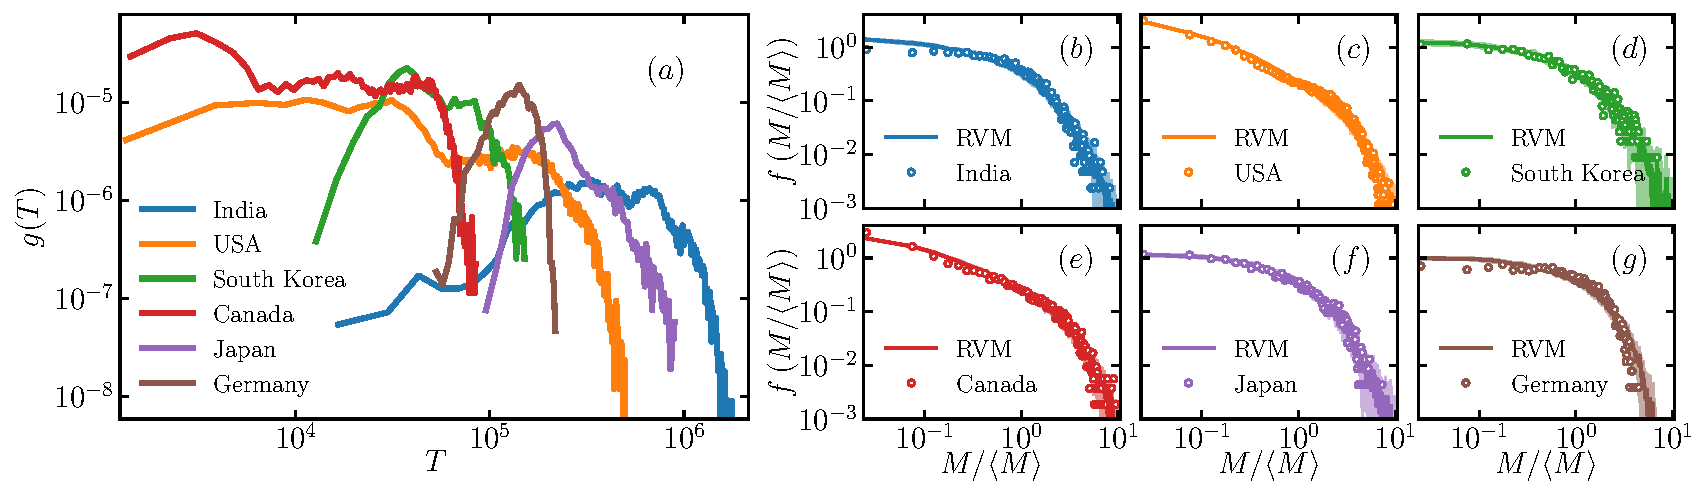
\includegraphics[width=\textwidth]{chapters/chapter4/fig_1.pdf}
    \caption{(a) Turnout distribution $g(T)$ obtained from election data for different countries. Note the differences in shapes and ranges for $g(T)$. (b-g) Scaled margin distribution $f(M/\langle M \rangle)$ obtained from election data (open circles) for India, USA, South Korea, Canada, Japan, and Germany. Despite their distinct electoral systems and political cultures, these distributions show broad similarities but also notable differences in their decay patterns.}
    \label{fig:turnout_margin}
\end{figure}

The corresponding scaled margin $M/\langle M \rangle$ is displayed as distribution $f(M/\langle M \rangle)$ (computed from the consolidated margin data for each country) in Fig.~\ref{fig:turnout_margin}(b-g). While they appear to be broadly similar, certain differences are clearly noticeable. In particular, $f(M/\langle M \rangle)$ for German elections in Fig.~\ref{fig:turnout_margin}(g) has a sharp cutoff, but for India and Japan in Fig.~\ref{fig:turnout_margin}(b, f) the distribution has a slower decay. These observations motivate the questions of whether $f(M/\langle M \rangle)$ is related to the raw turnout distribution and can be obtained from it.

\section{The Universality Landscape: Scope and Robustness}

A robust universal pattern must hold across different scales of electoral units. In large countries, depending on the size of the electoral unit, the typical turnout can differ by several orders of magnitude. For instance, in India, polling booths have a typical electoral size of around $10^3$ voters, whereas at the parliamentary constituency level, it is approximately $10^6$ voters—a thousand-fold difference in scale.

Next, we show that these results are independent of the number of voters or size of electoral units. In large countries, depending on the size of the electoral unit, the typical turnout can differ by several orders of magnitude. For example, in India, polling booths have a typical electoral size $\sim 10^3$, whereas, at the parliamentary constituency level, it is about $10^6$. Further, the shapes of $g(T)$ are also vastly different at different scales. Figure \ref{fig:scale_independence}$(a)$ captures the striking differences in range and shape of $g(T)$ for India, the US, and Canada at two different scales. The dashed lines represent smaller scales (polling booths for India and Canada, counties for the USA), while solid lines represent larger scales (constituencies for India and Canada, congressional districts for the USA).

\begin{figure}[H]
    \centering
    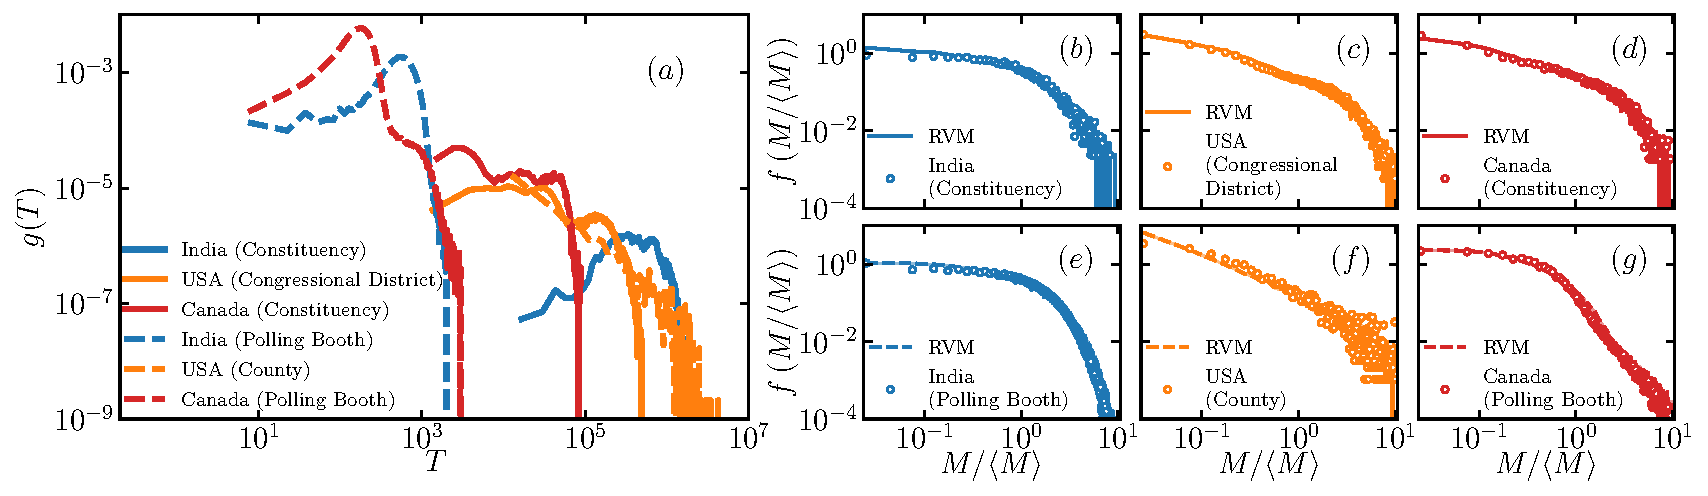
\includegraphics[width=\textwidth]{chapters/chapter4/fig_2.pdf}
    \caption{The turnout distribution $g(T)$ and scaled margin distribution $f(M/\langle M \rangle)$ for India (blue), the USA (orange), and Canada (red), at two widely different scales, {\it i.e.}, size of electoral units. (a) $g(T)$ at two different scales for each country. The dashed line is for smaller scales (polling booth for India and Canada, County for the USA), while the solid line represents a larger scale (constituency for India and Canada, congressional district for the USA). (b-g) $f(M/\langle M \rangle)$ from election data (open circles). Despite the differences in scale and shape of $g(T)$, the empirical $f(M/\langle M \rangle)$ shows certain consistent patterns, though scale effects are still evident.}
    \label{fig:scale_independence}
\end{figure}

The corresponding scaled margin distributions $f(M/\langle M \rangle)$ are shown in Figure \ref{fig:scale_independence}(b-g). Figure \ref{fig:scale_independence}$(b, c, d)$ shows the empirical distribution of scaled margins (in national elections) at the constituency-level scale, and Figure \ref{fig:scale_independence}$(e, f, g)$ shows the same at the scale of polling booths (county for USA). For each country, the distributions at different scales show certain similarities but also notable differences. For instance, in the USA, the county-level distribution (Figure \ref{fig:scale_independence}(f)) displays a heavier tail compared to the congressional district level (Figure \ref{fig:scale_independence}(c)), reflecting the influence of the underlying turnout distribution. Similar scale-dependent effects are visible in the data from India and Canada.

This is particularly evident for the USA, where the county-level turnout distribution shows a heavy-tailed decay, which is reflected in the corresponding scaled margin distribution (Fig.~\ref{fig:scale_independence}(f)). The faster decay at congressional district level distribution (Fig.~\ref{fig:scale_independence}(c)) is also observed. For Canada too, the empirical scaled margin distributions are noticeably different at two different scales. 

These observations suggest that while the scaled margin $M/\langle M \rangle$ brings us closer to universality than raw margins, it still carries the imprint of the underlying turnout distribution and is affected by the scale of electoral units. This motivates us to seek a more fundamental measure that might transcend these differences.

\section{The "Aha!" Moment: The Scaled Margin-to-Turnout Ratio}

Given the observed dependencies between margins and turnouts, and the constraint that $M \leq T$, we consider a new measure: the specific margin $\mu = M/T$. This ratio represents the margin normalized by the turnout at each electoral unit, producing a dimensionless measure of electoral competitiveness that is independent of the size of the electorate. This is a turnout-independent measure of electoral competitiveness and does not depend on the size of the electorate.

The specific margin $\mu$ ranges from 0 to 1, where values close to 0 indicate extremely competitive elections (nearly tied results), and values approaching 1 represent complete consensus (where nearly all voters chose the same candidate). By normalizing the margin by the local turnout, we effectively remove the scale dependency that affected our earlier analysis.

\subsection{Universal Distribution of Scaled Specific Margin}

The true breakthrough comes when we examine the scaled specific margin $x = \mu/\langle\mu\rangle$, where $\langle\mu\rangle$ is the average specific margin for each country. Figure \ref{fig:universality}(b) shows the distribution $F(x)$ of this scaled specific margin computed from electoral data across 32 countries.

\begin{figure}[H]
    \centering
    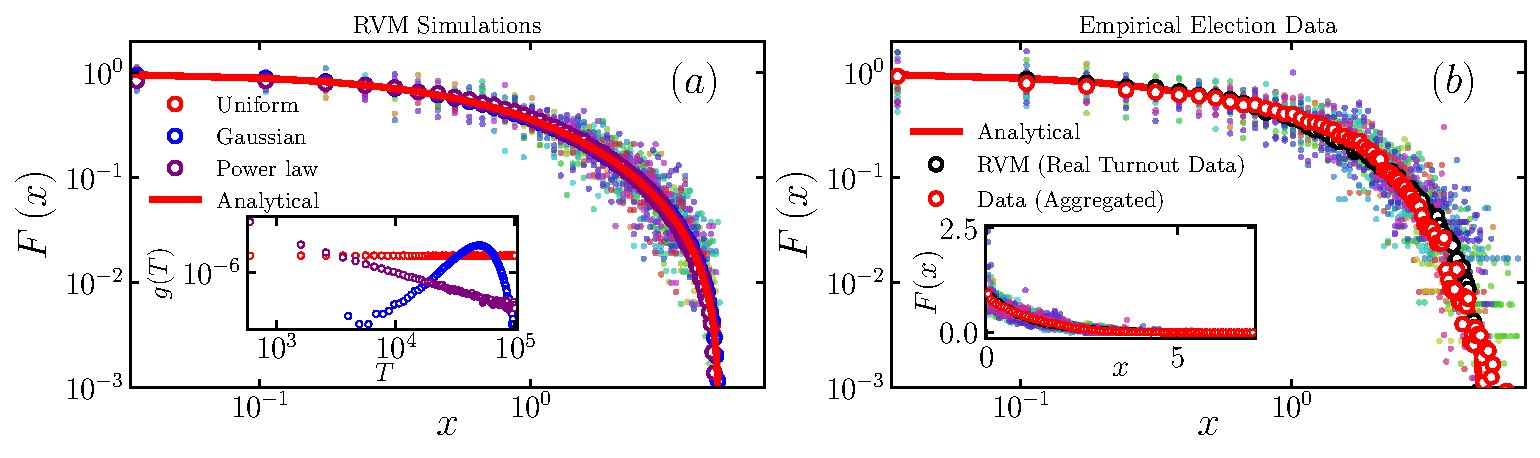
\includegraphics[width=\textwidth]{chapters/chapter4/fig_3.pdf}
    \caption{(a) Distributions of scaled specific margin $x=\mu/\langle\mu\rangle$ for different initial distributions (inset). Despite different initial distributions, a common pattern emerges. (b) The empirical distribution of $x=\mu/\langle \mu \rangle$ from election data of 32 countries (excluding Ethiopia and Belarus). Each color indicates a specific country for which the empirical election data is consolidated over several elections. The average of these empirical distributions (red open circles) reveals a striking universality. The inset depicts the distributions on a linear scale.}
    \label{fig:universality}
\end{figure}

Remarkably, Figure \ref{fig:universality}(b) reveals that the distribution $F(x)$ collapses onto a single universal curve across all 32 countries, despite vast differences in their electoral systems, cultural contexts, and historical backgrounds. Each colored point in the figure represents a specific country's data, and while there are small fluctuations around the universal curve (attributable to finite-size effects), the overall pattern is strikingly consistent. The average of all these empirical distributions, shown as red open circles, follows a smooth curve that appears to be independent of country-specific details.

The empirical distribution for each of the $32$ countries (denoted by the solid-colored circles) closely follows the trend of $F(x)$, albeit with some fluctuations induced by the finite size of data. Empirical distributions shown in the inset of Fig.~\ref{fig:universality}(b) demonstrate that at large $x$, the absolute fluctuations decrease. 

This represents a profound discovery: despite the immense complexity and diversity of electoral systems worldwide, the scaled specific margin follows a universal distribution. This suggests that the fundamental process of electoral competition—when appropriately normalized—follows the same statistical pattern regardless of where or how the election takes place.

\section{The Challenge: Can We Explain This Universality?}

While the empirical universality we've discovered is compelling, it raises a fundamental question: Why does this universal pattern emerge across such diverse electoral systems? What underlying mechanism could generate such consistent statistical behavior despite the vast differences in political contexts, voter behaviors, and electoral rules?

To obtain analytical insight, we can consider elections with three candidates in the limit of large turnout ($T \gg 1$). The votes received by $j$-th candidate can be approximated as $v_j \approx p_jT$, and the margin as $M \approx \left(p_{(3)} - p_{(2)}\right) T$, where $p_{(k)}$ denotes $k$-th order statistics of the probabilities assigned to the candidates. Evidently, in this limit, $\mu \approx p_{(3)} - p_{(2)}$ and its distribution has no explicit dependence on $T$. With this insight, the distribution of specific margins can be expressed as:

\begin{equation}
    P(\mu) = \frac{(1 - \mu)(5 + 7\mu)}{(1 + \mu)^2(1 + 2\mu)^2}
\end{equation}

Thus, the distribution $F(x)$ of the scaled specific margin $x = \mu/\langle\mu\rangle$ is:

\begin{equation}
    F(x) = \langle\mu\rangle P(x\langle\mu\rangle)
\end{equation}

with $\langle\mu\rangle = \frac{1}{2} + \ln\left(\frac{9\sqrt[4]{3}}{16}\right)$.

Remarkably, this distribution is independent of the details of the turnout distribution $g(T)$. This explains why the empirical data from vastly different countries collapses onto a single curve—the underlying statistical pattern transcends the specifics of any particular electoral system or turnout pattern.

The universality in Fig.~\ref{fig:universality} suggests that irrespective of the finer details of election processes, the mechanism underlying the core component of any competitive election -- choosing one candidate from many contenders -- leads to a universal distribution for the scaled specific margin $x=\mu/\langle \mu \rangle$.

\subsection{A Glimpse of the Mechanism: Setting Up the Random Voting Model}

The consistency of the pattern suggests that there might be a simple but powerful statistical principle at work—something fundamental to the process of competitive selection itself, rather than specific to electoral politics. The universality we've discovered hints that once turnout is "normalized out" through the specific margin, what remains is a fundamental statistical process common to all competitive elections. 

This suggests that a minimal model focused on the core statistical features of electoral competition might be sufficient to explain the observed universality. Such a model would need to capture the essential statistical features of electoral competition without relying on detailed assumptions about voter psychology, campaign dynamics, or specific electoral rules. Instead, it would focus on the basic structure of competitive selection processes, where multiple candidates compete for a finite number of votes.

In the next chapter, we will introduce precisely such a model—the Random Voting Model (RVM)—which explains this universality from first principles and makes additional predictions about electoral statistics across different scales and contexts. This parameter-free model demonstrates how the distribution of margins is fundamentally driven by the turnout distribution, yet the scaled specific margin follows a universal pattern independent of turnout.

\section{Conclusion: Universality as a Signature of Democratic Competition}

In this chapter, using extensive election data from 34 countries spanning multiple decades and electorate scales, we have demonstrated universality through analysis of the margin of victory and turnout data in democratic elections. We have shown that while raw turnout distributions vary dramatically across countries and scales, and scaled margin distributions retain country-specific features, the scaled specific margin follows a universal distribution across 32 diverse democracies.

This universality transcends the particularities of individual countries, electoral systems, and scales, revealing a fundamental statistical signature that appears to be intrinsic to competitive democratic processes. Like other universalities discovered in complex systems, this pattern emerges not despite but because of the underlying complexity, as the central limit theorem emerges from the aggregation of many random variables.

Competitiveness in any election is encoded in the victory margins and turnouts. The latter also expresses people's interest in the participatory democratic process. The scaled distribution of margin-to-turnout ratio $\mu$ has a universal form for all elections independent of country, regions, turnouts and the scale of elections. This result can be regarded as a stylized fact of elections. 

The universal distribution we've identified should be considered a stylized fact of democratic elections—an empirical regularity that any successful election model must reproduce. In the next chapter, we will develop precisely such a model, demonstrating how a simple yet powerful framework can explain this universality and make additional predictions about electoral statistics across different scales and contexts.
